\subsection{Results and discussion}\label{sec:m3:results}
    
    ~\cref{fig:m3:potentials} shows the metric perturbation potentials $\Phi$ and $\Psi$ as functions of time $x$ for the $k$-modes under investigation. The time of matter-radiation equality and recombination is marked in the plot as black dash-dotted and dashed lines respectively. Let's first consider the top panel, showing only $\Phi$. At early times, it seems to be constant across all $k$-modes. \footnote{When referring to ``all $k$-modes'' it is implicit that we only mean the three modes considered here, but the qualitative discussions should be valid across all $k$-modes.} This is expected since at early times, the horizon is small and most modes are larger than this. Thus, they will be unaffected by causal physics and stay constant at their initial value. As time proceeds, the smaller $k$-modes will be surpassed by the horizon and are suddenly subjected to causal physics. We see from the top panel that if this happens in the radiation dominated regime (before radiation-matter equality), the potential will decline as $e^{-2x}$. This can be seen from ~\cref{eq:m3:theory:phi_perturbation}. The sum of the potentials in the bottom panel of ~\cref{fig:m3:potentials} goes as $\Psi+\Phi \sim e^{-2x}/k^2\T_2$, so it will closely follow the quadrupole term, but being suppressed by an exponential factor. Also, the $k^2$ term suggested larger value for small $k$-s (large scale). We save the discussion of the quadrupole, but the latter can clearly be seen as the large and intermediate scale modes show sinusoidal behaviour, with the large scale mode having a larger amplitude. Both are exponentially suppressed. These effects happen when the tight coupling epoch is over, since all multipoles except the monopole and dipole are suppressed during tight coupling. 
    \begin{figure}
        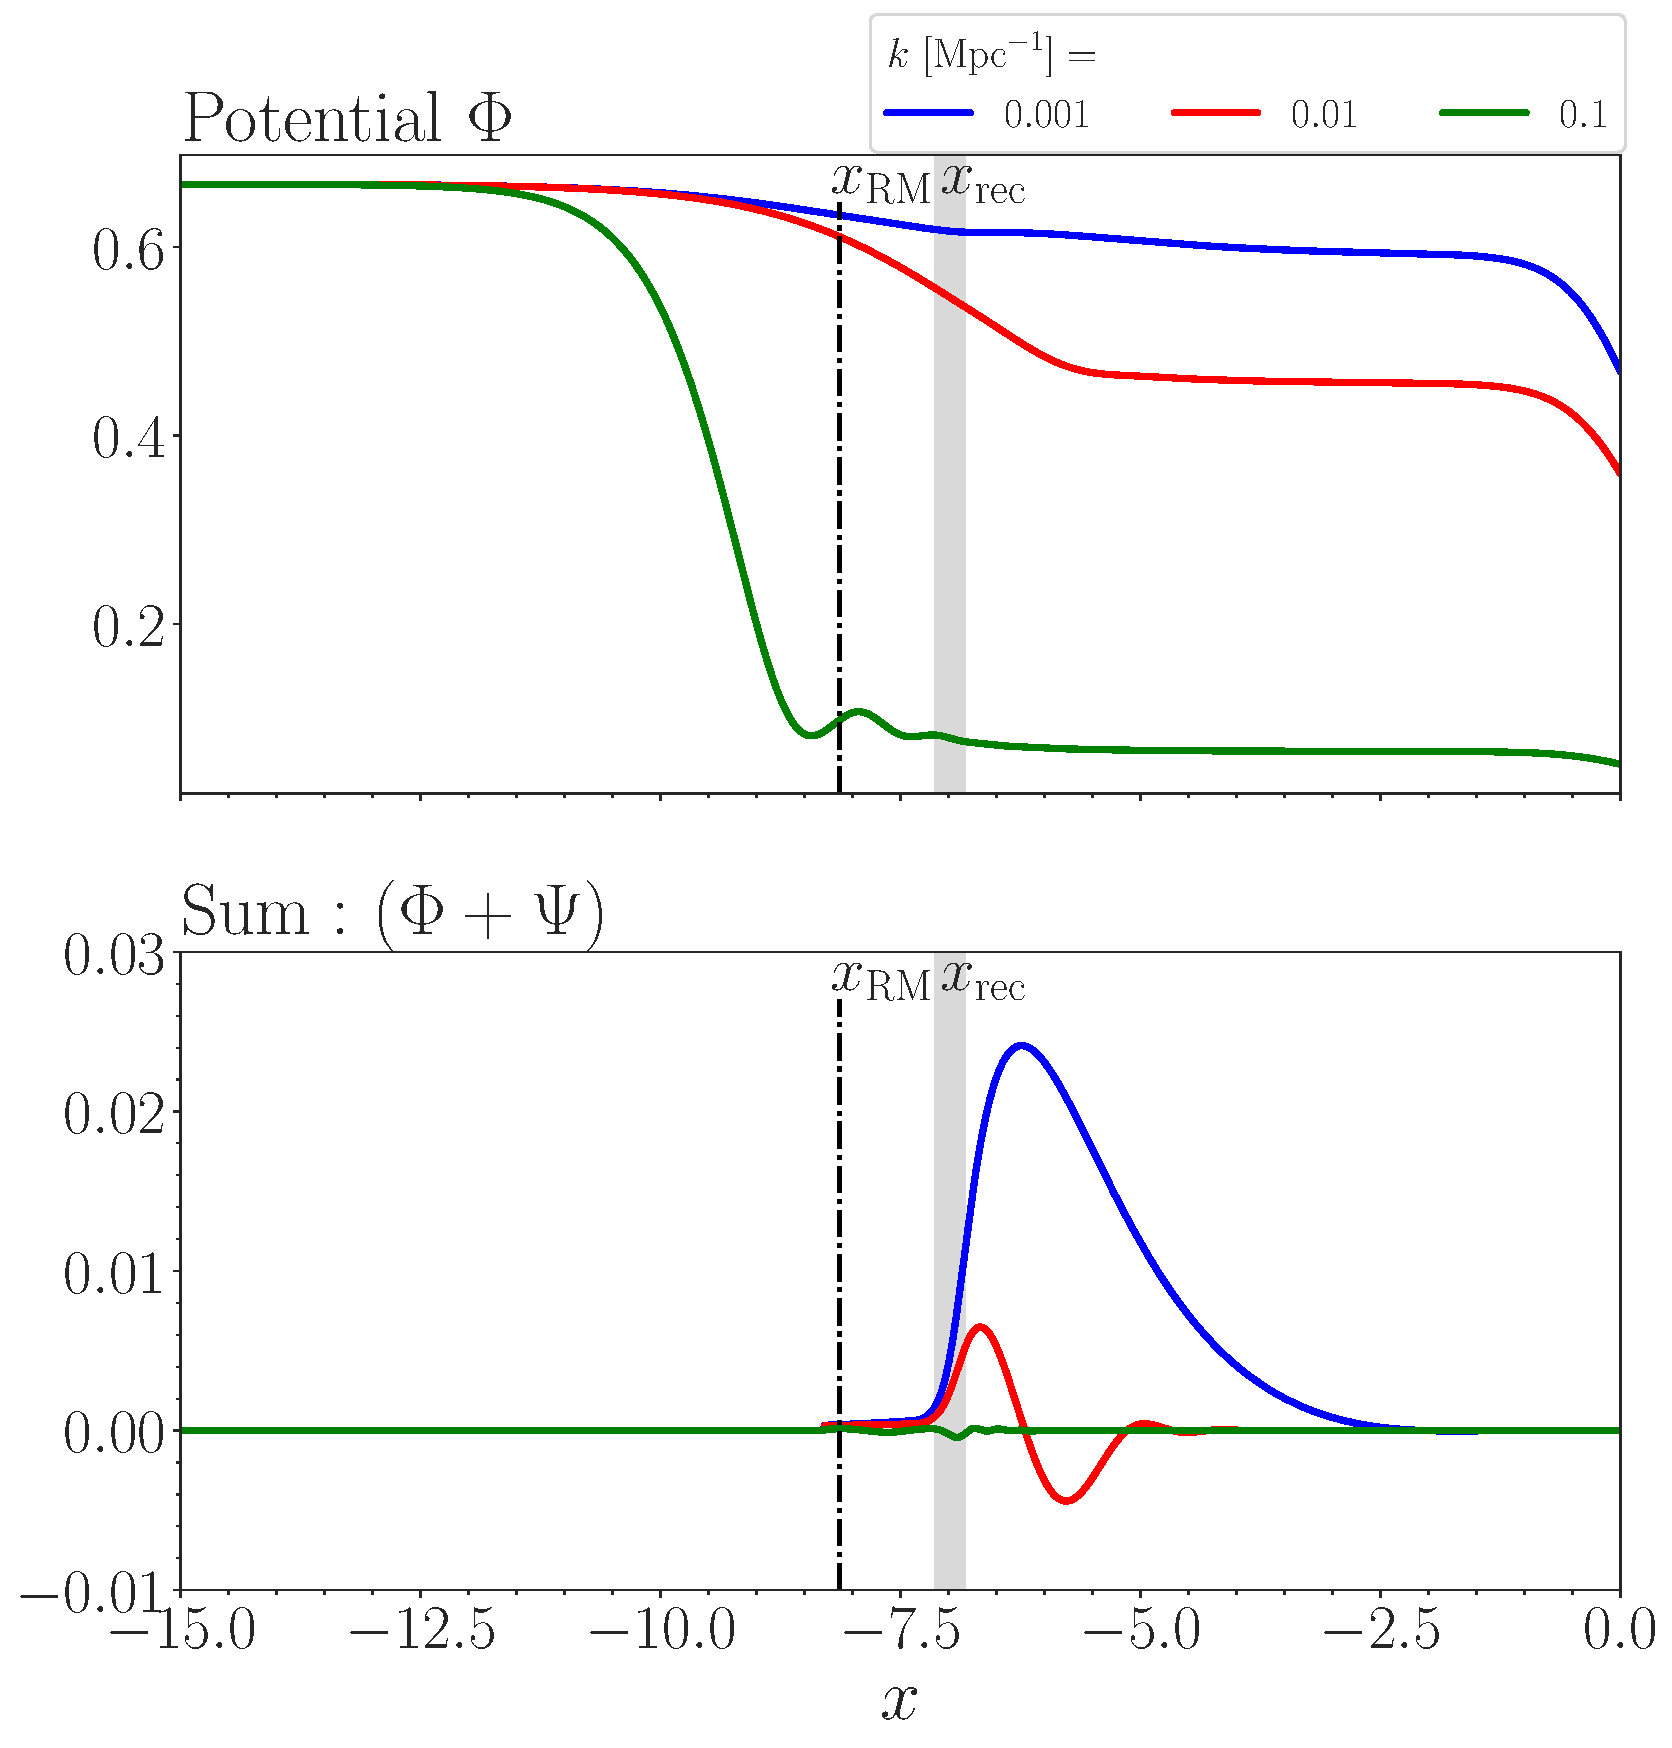
\includegraphics[width=\linewidth]{potentials.pdf}
        \caption{The metric perturbation potentials, $\Psi$ representing the Newtonian potential, and $\Phi$ representing the spatial curvature perturbations. Both panels show the evolution as function of the time $x$, for the three different $k$-modes outlined in ~\cref{sec:m3:methods}. The top panel shows $\Phi$ alone, while the bottom shows the sum of the two. The dashed black line is the time of recombination as found in ~\cref{sec:m2}, and the dash-dotted black line is the time of radiation-matter equality as found in ~\cref{sec:m1}.}
        \label{fig:m3:potentials}
    \end{figure}

    We now focus our attention on the multipoles, starting with the monopole term expressed through the photon overdensity $\delta_\gamma = 4\T_0$. Mathematically, this relation can be seen  from either the parenthesis in ~\cref{eq:m3:theory:time_evolution_of_Phi} or the definition of $\mathcal{Y}$ in ~\cref{eq:m3:theory:metric_perturbations_final} following somewhat diffuse symmetry arguments. Physically it also makes sense since the photon monopole is some measure of the average photon temperature which intuitively can be though of as a photon overdensity. It can be seen for the various $k$-modes in ~\cref{fig:m3:monopole}, where we clearly see that the small scale perturbation undergoes horizon crossing first, and become subject to causal physics. This is manifest in the oscillation of the green curve in the figure. Metric perturbations and pressure will generate acoustic oscillations within causally connected regions. When the horizon increase, these oscillations will affect a spatially large area, affecting $k$-modes on larger and larger scales. This is also manifest in ~\cref{fig:m3:monopole} as the intermediate $k$-mode starts to oscillate later, and finally the large scale mode. 
    \begin{figure}
        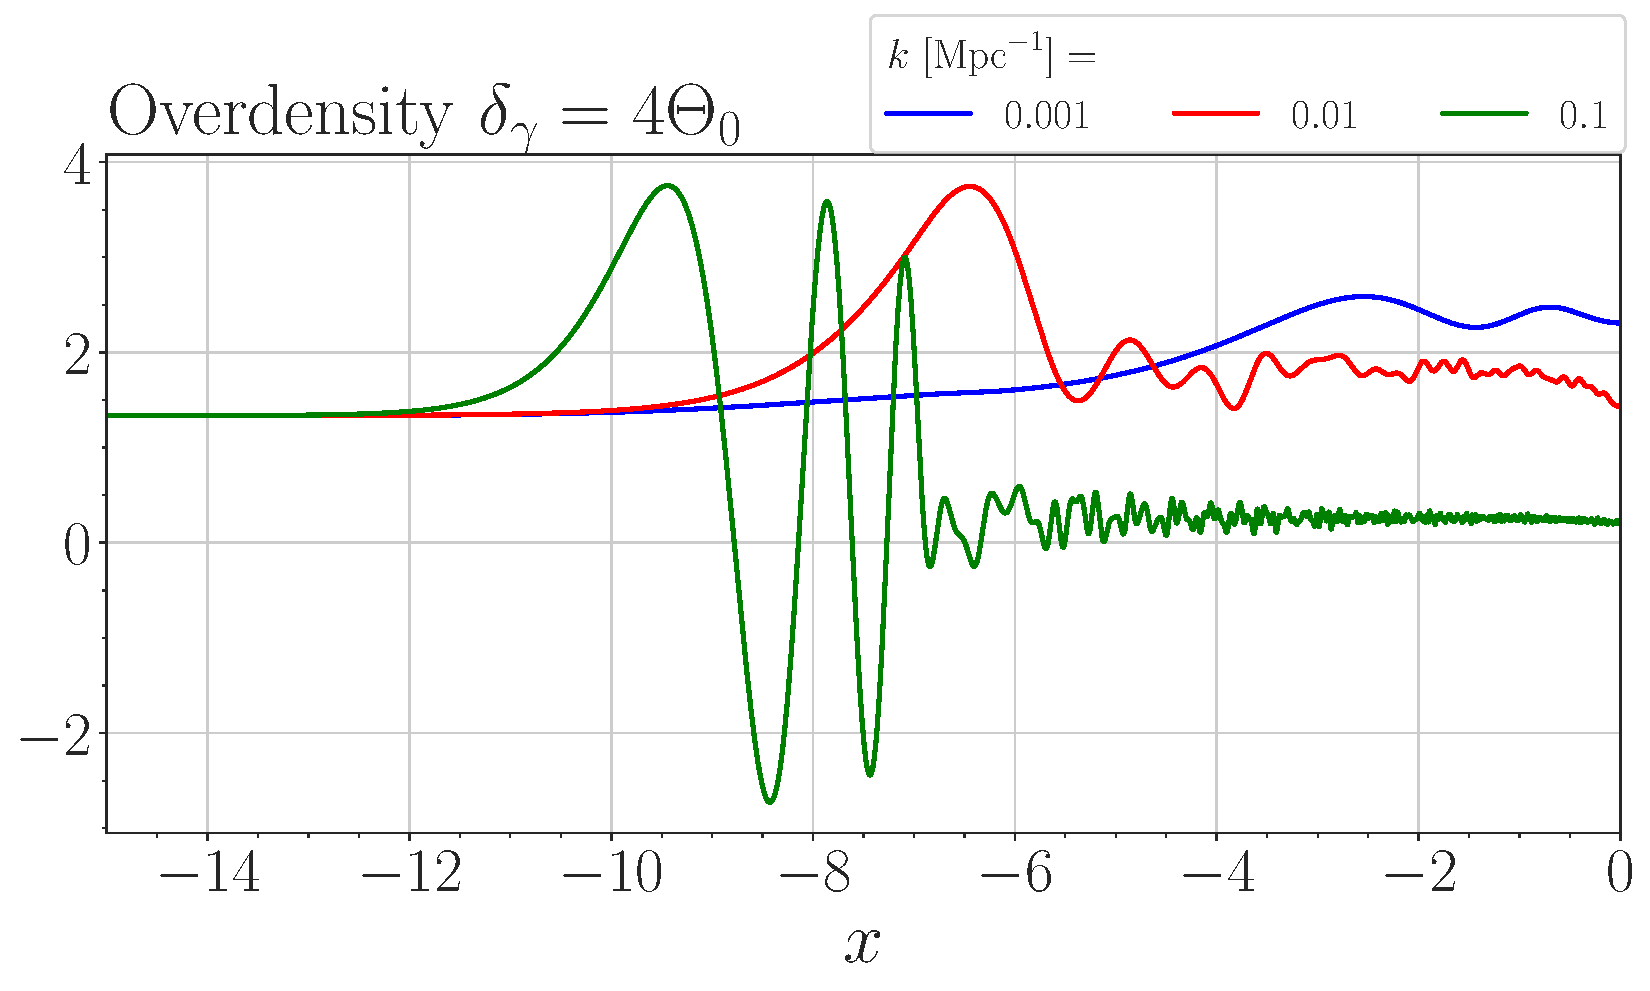
\includegraphics[width=\linewidth]{monopole.pdf}
        \caption{Monopole term The dashed black line is the time of recombination as found in ~\cref{sec:m2}, and the dash-dotted black line is the time of radiation-matter equality as found in ~\cref{sec:m1}.}
        \label{fig:m3:monopole}
    \end{figure}

    \begin{figure}
        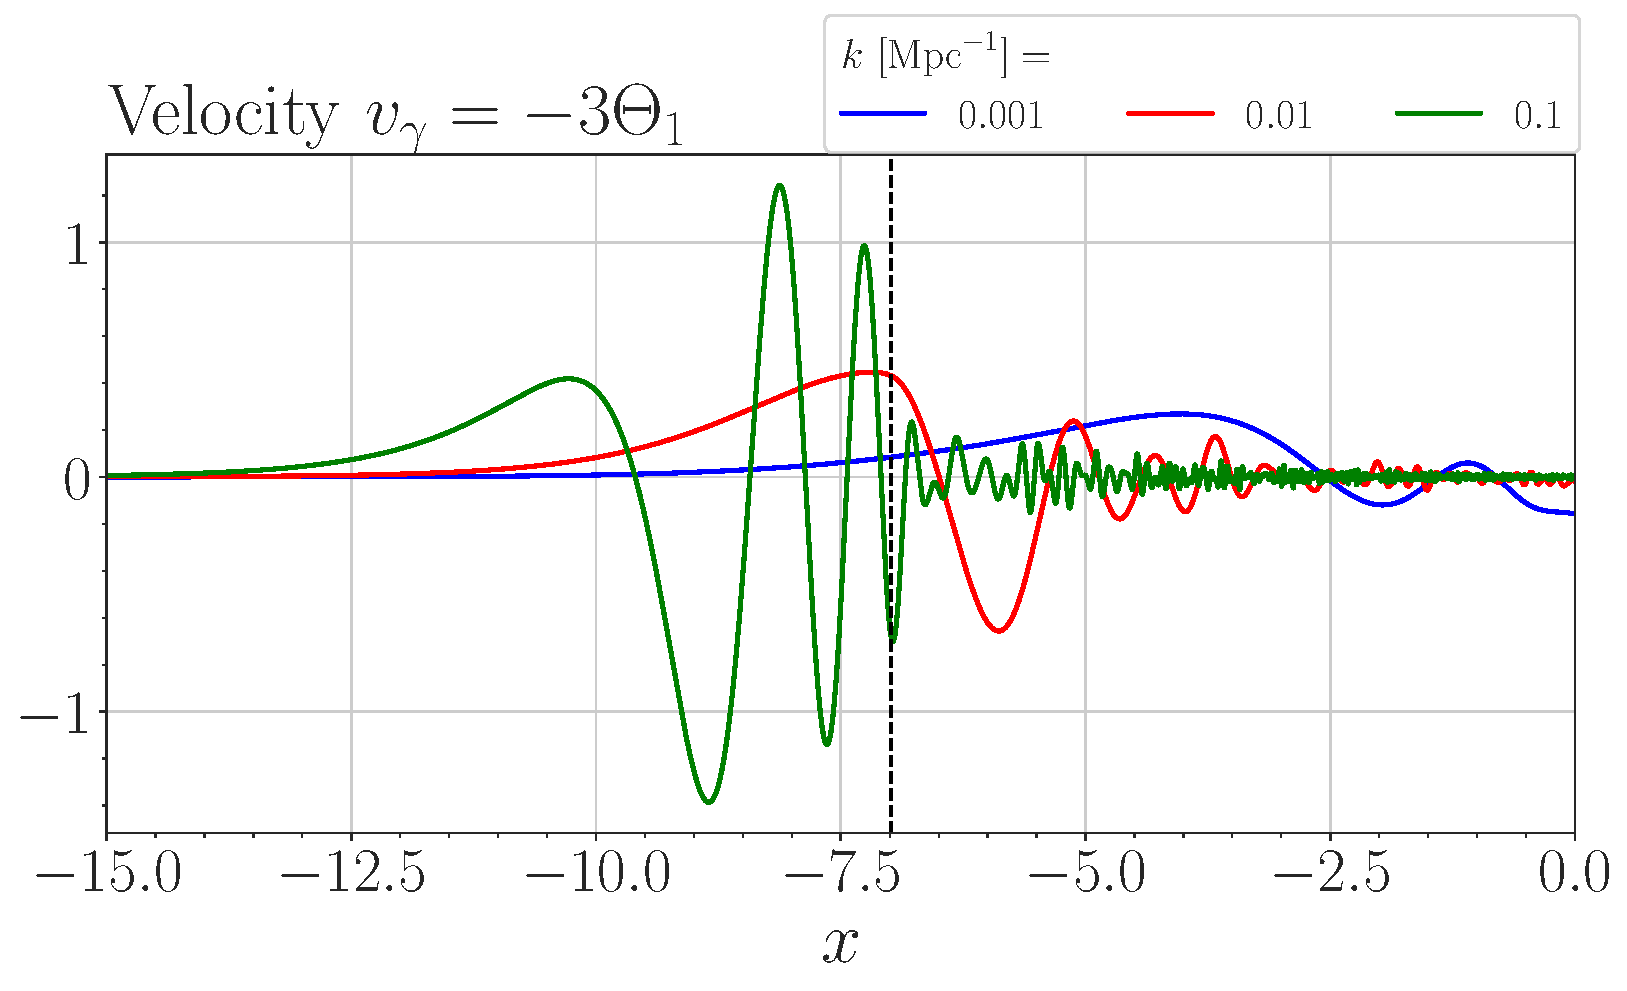
\includegraphics[width=\linewidth]{dipole.pdf}
        \caption{Dipole term The dashed black line is the time of recombination as found in ~\cref{sec:m2}, and the dash-dotted black line is the time of radiation-matter equality as found in ~\cref{sec:m1}.}
        \label{fig:m3:dipole}
    \end{figure}

    \begin{figure}
        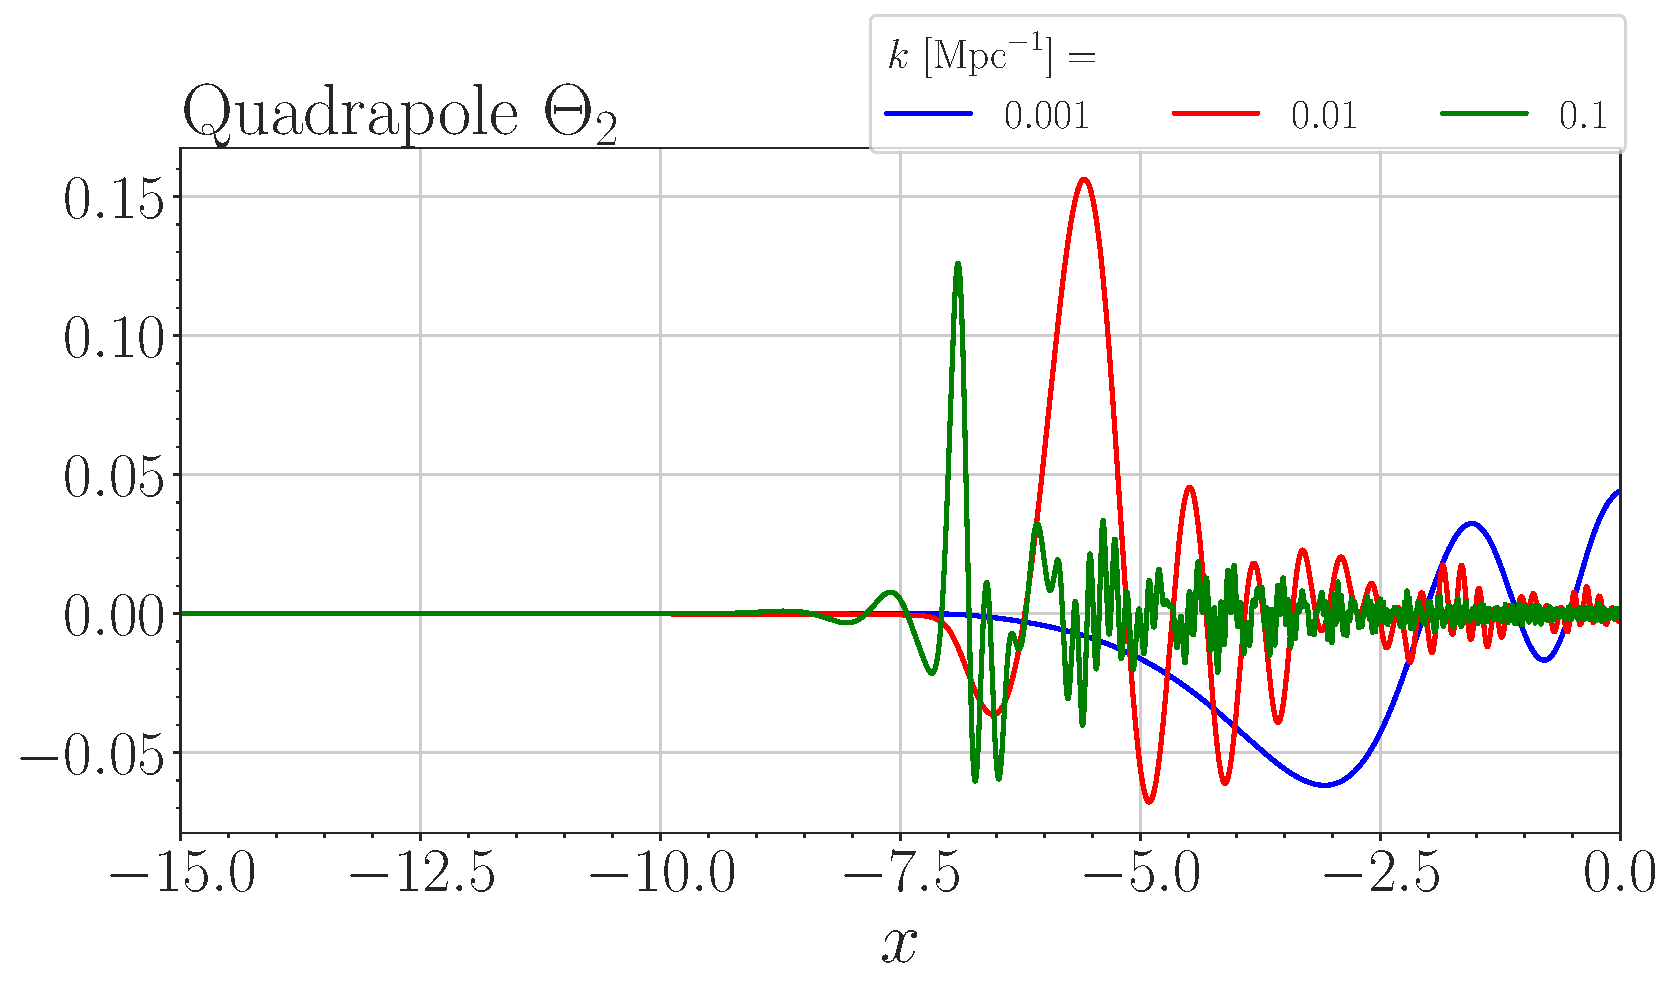
\includegraphics[width=\linewidth]{quadrapole.pdf}
        \caption{Quadrapole term The dashed black line is the time of recombination as found in ~\cref{sec:m2}, and the dash-dotted black line is the time of radiation-matter equality as found in ~\cref{sec:m1}.}
        \label{fig:m3:quadrapole}
    \end{figure}

    \begin{figure}
        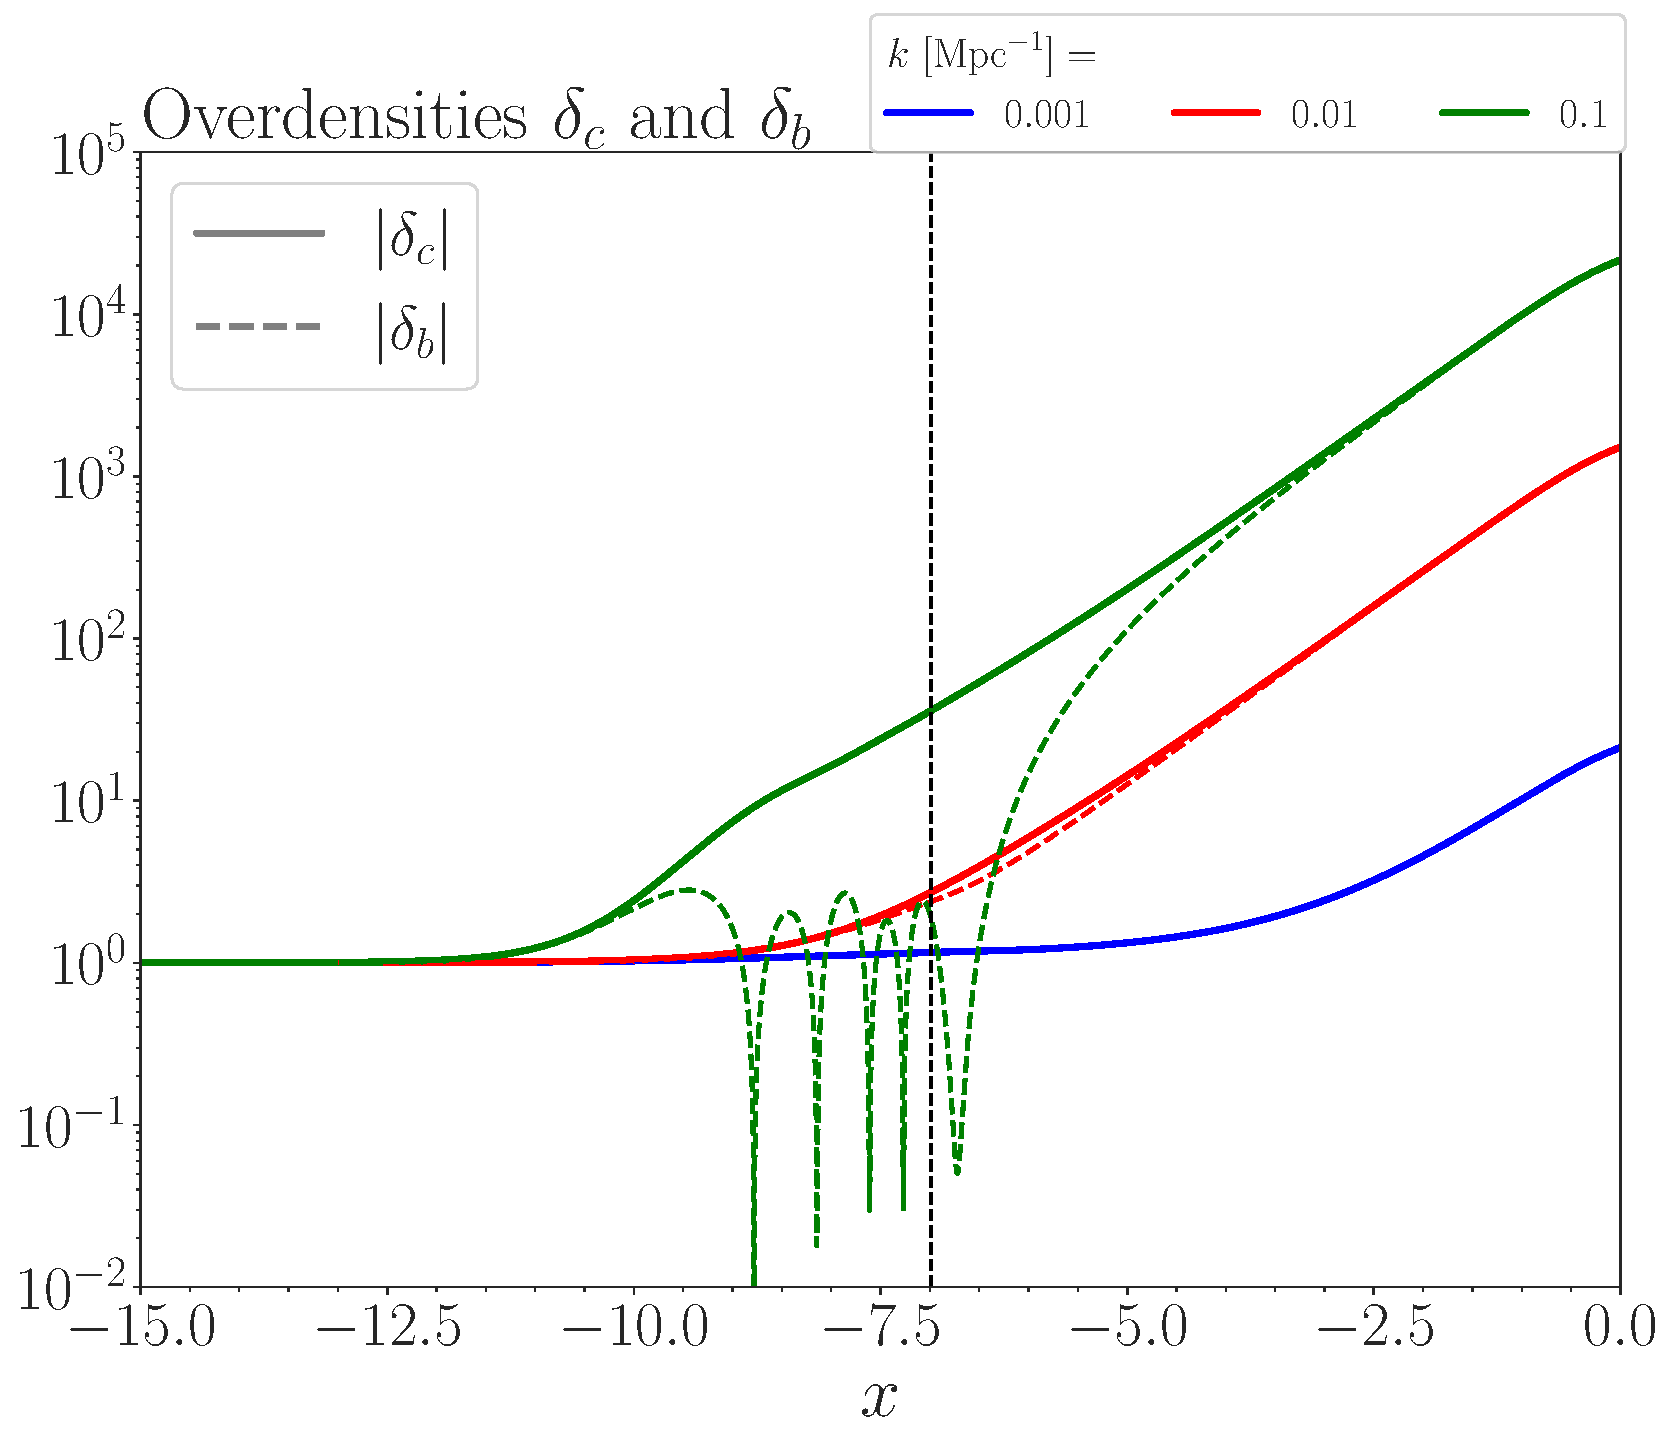
\includegraphics[width=\linewidth]{delta.pdf}
        \caption{delta term}
        \label{fig:m3:delta}
    \end{figure}

    \begin{figure}
        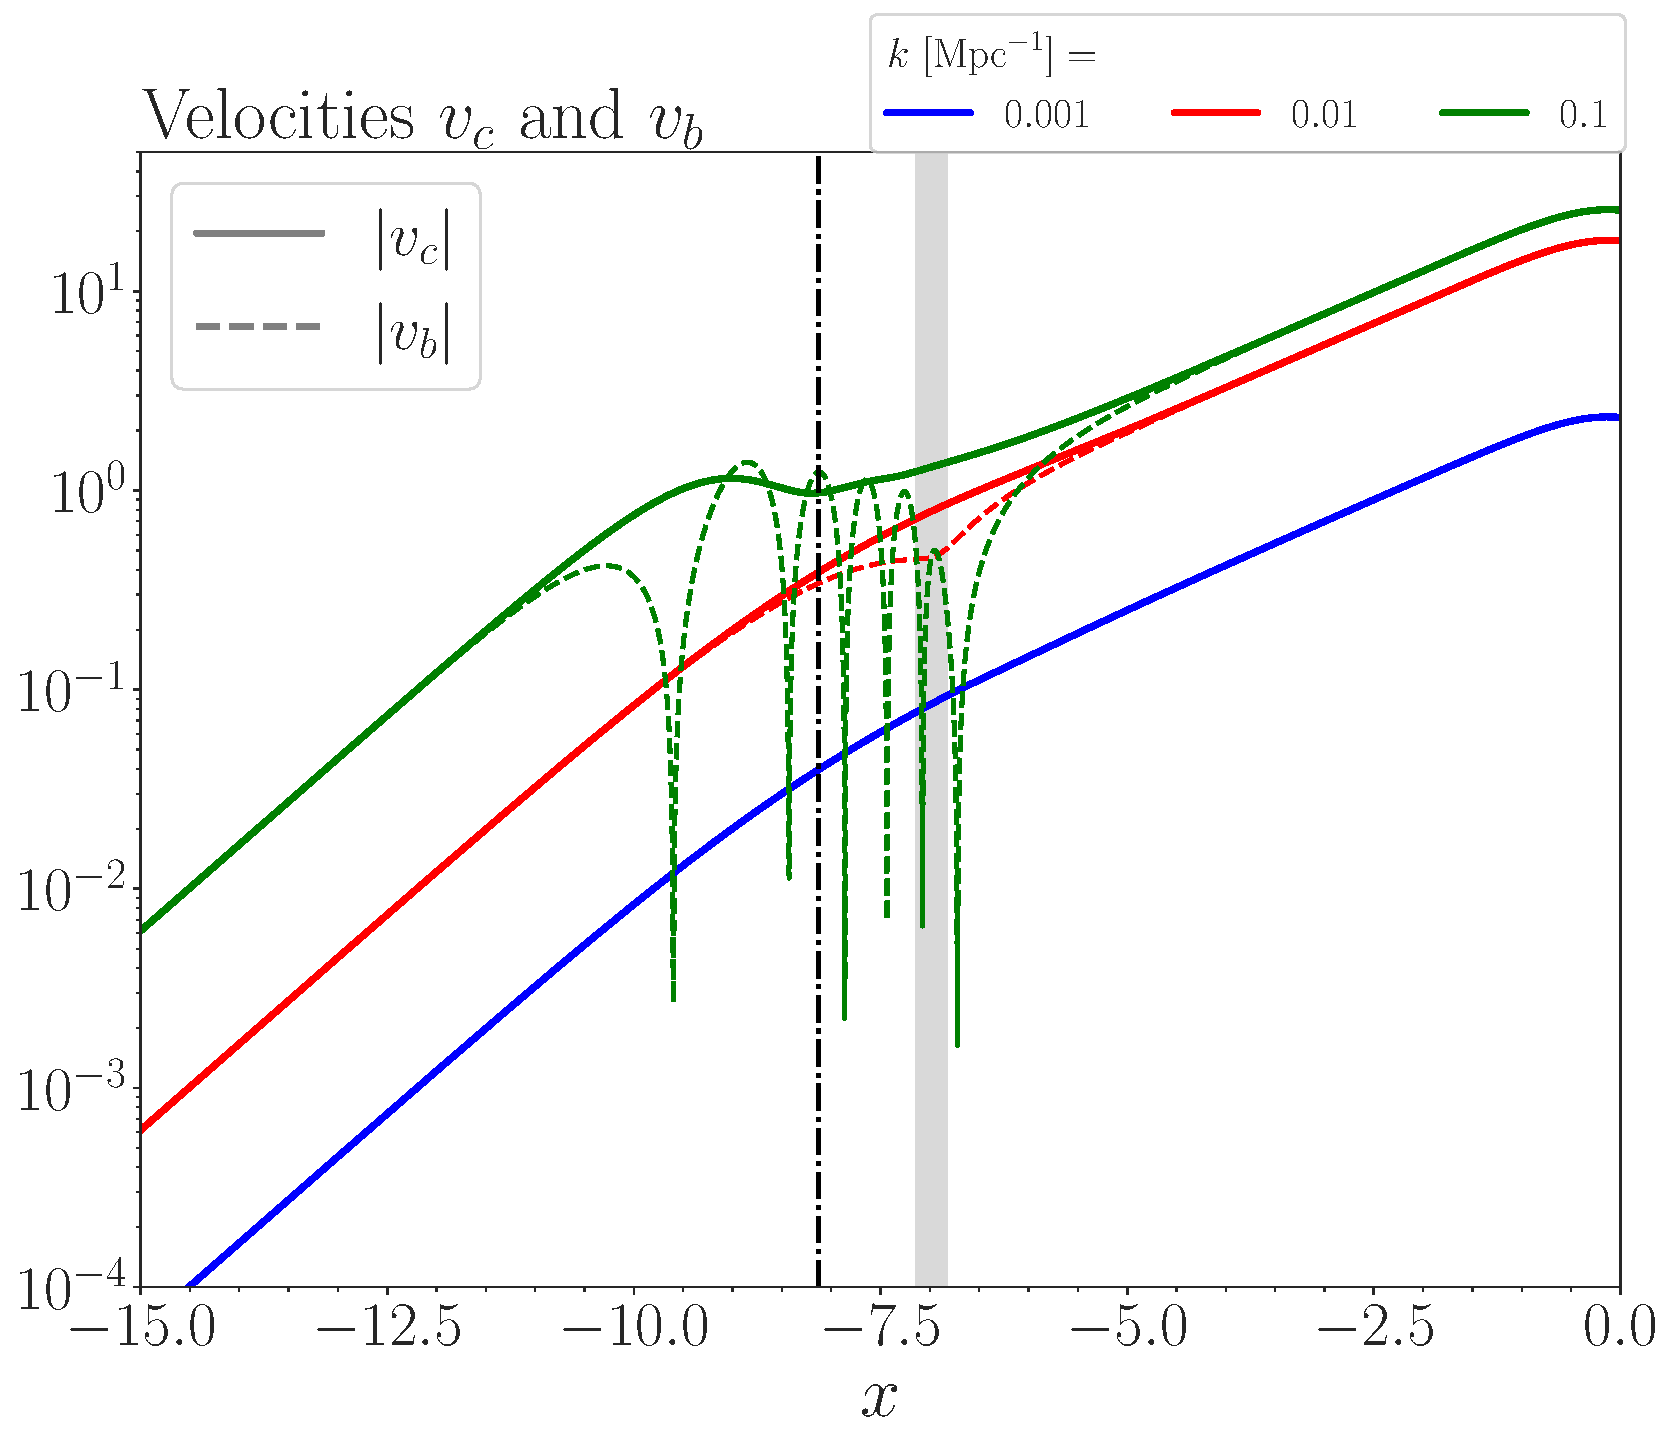
\includegraphics[width=\linewidth]{velocity.pdf}
        \caption{Velocities term}
        \label{fig:m3:velocity}
    \end{figure}

    \begin{figure}
        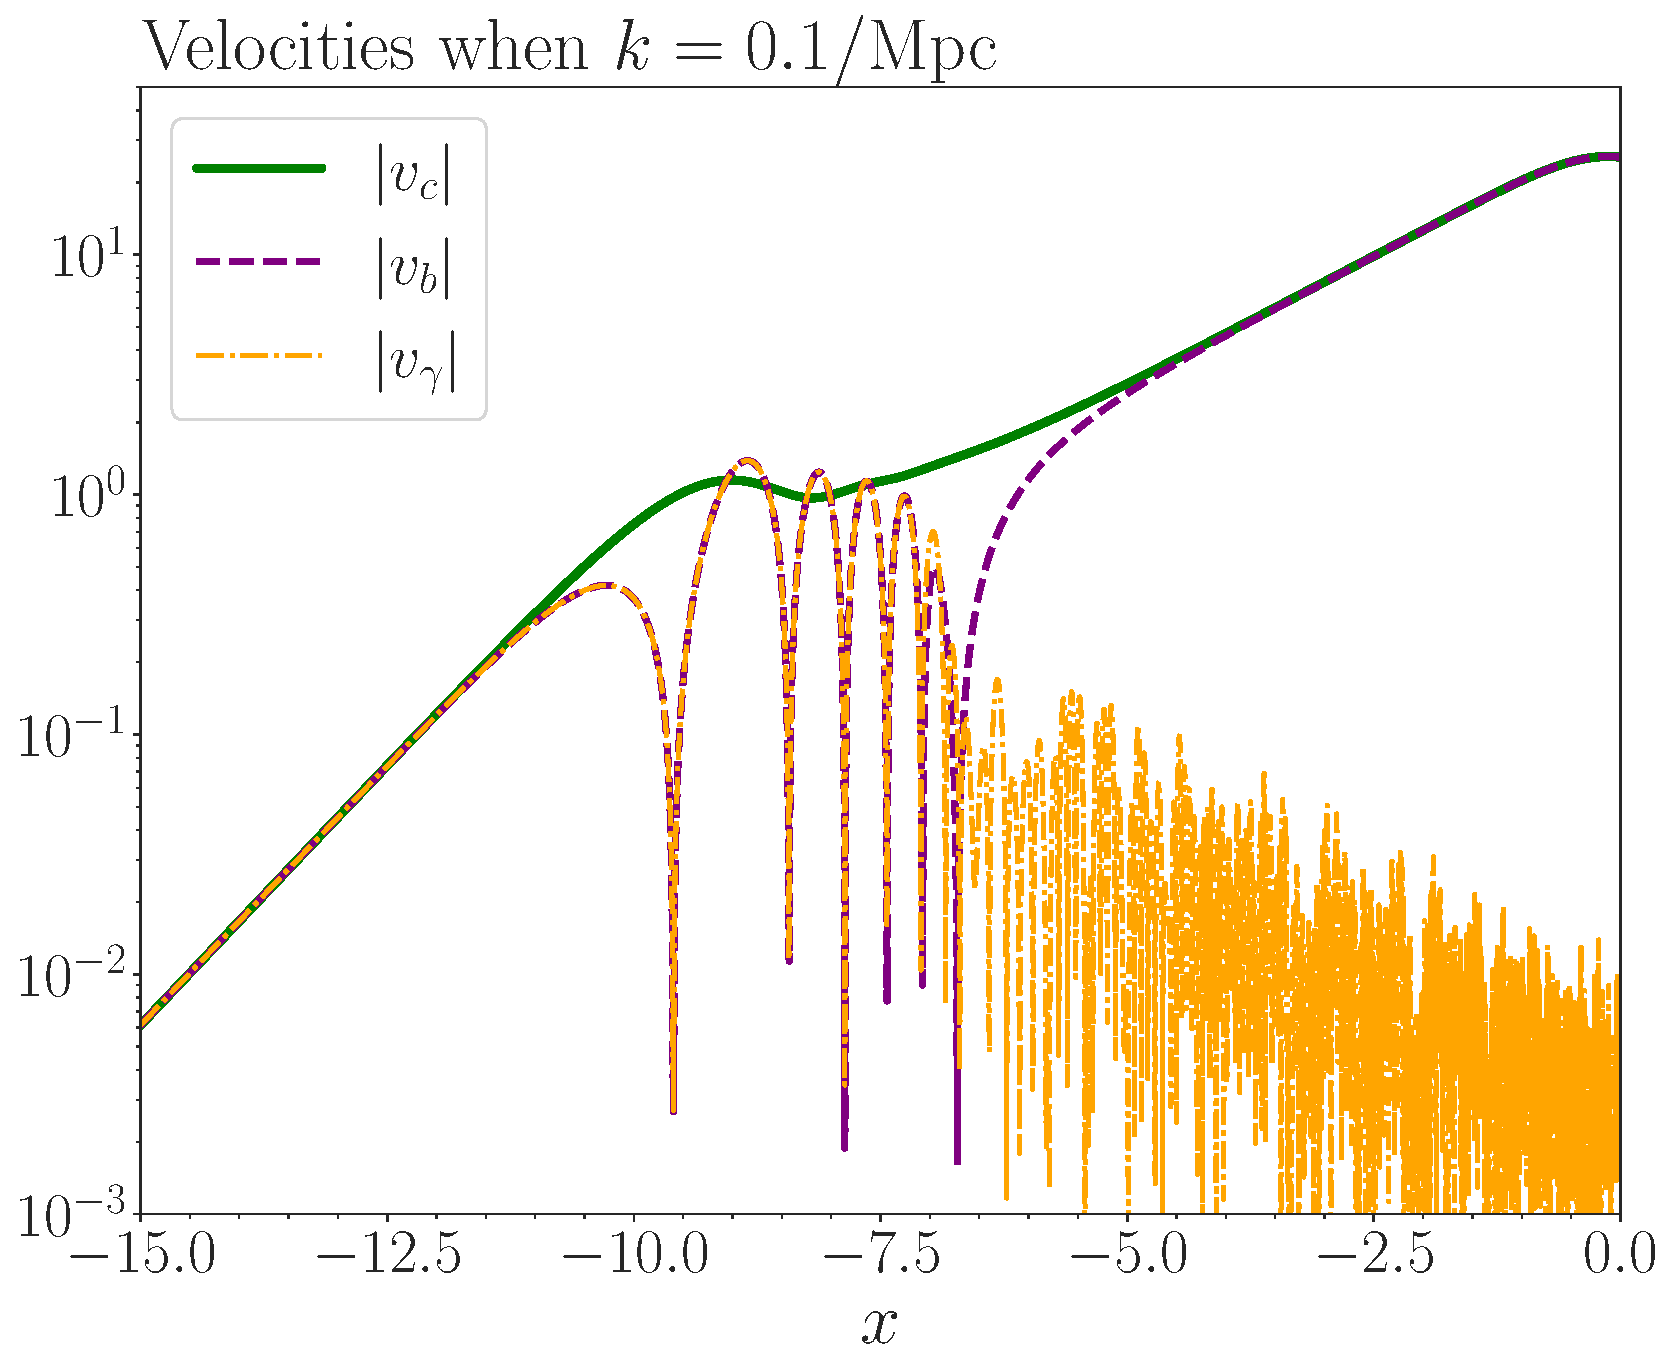
\includegraphics[width=\linewidth]{velocity_comparison.pdf}
        \caption{Velocities term}
        \label{fig:m3:velocity_comparison}
    \end{figure}

    \begin{figure}
        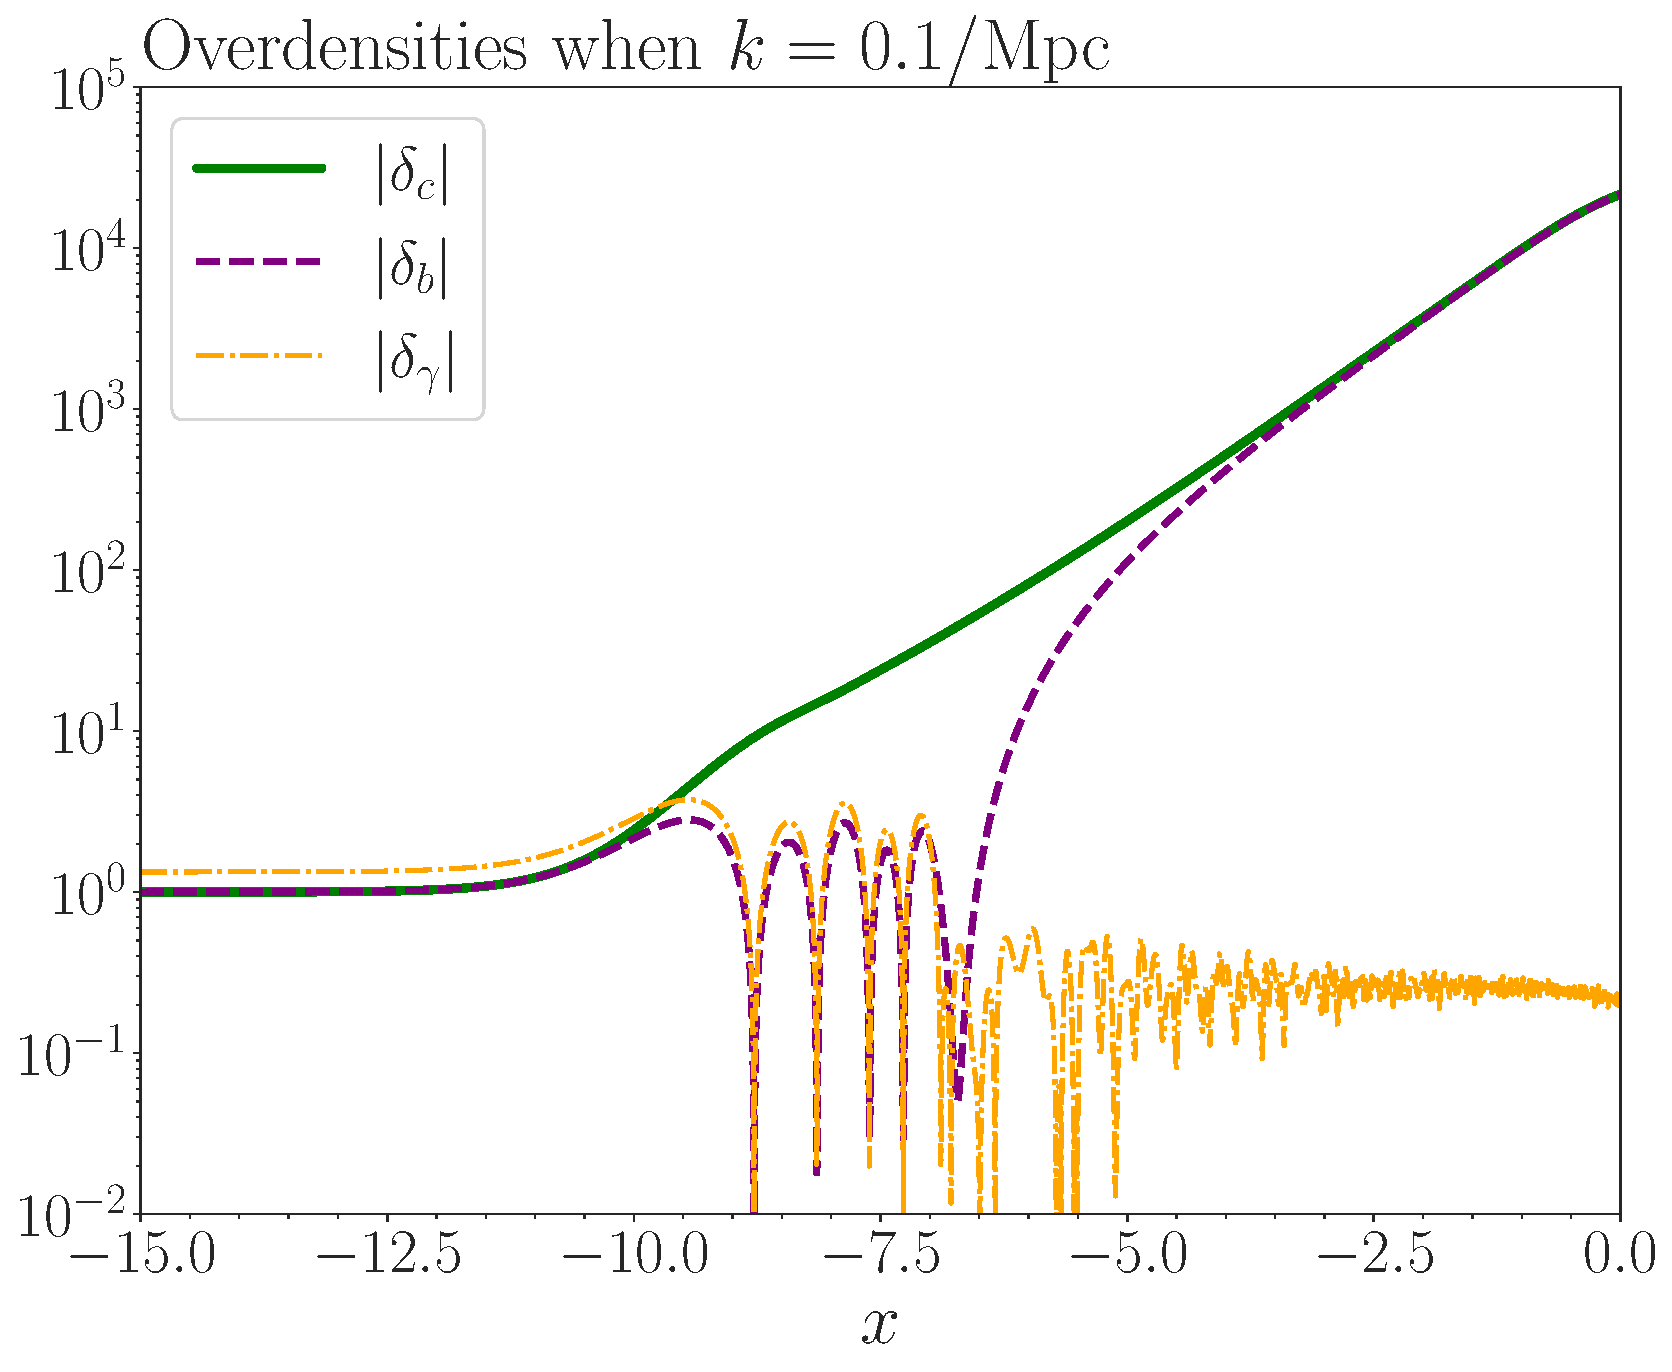
\includegraphics[width=\linewidth]{delta_comparison.pdf}
        \caption{Velocities term}
        \label{fig:m3:delta_comparison}
    \end{figure}

